\section{Dynamic Domain Assignment}
Thus, the routing 
configurations generated must adhere to 
these constraints. We describe the constraints
supported by the framework, points 1-4 are 
hard constraints we would ensure, while 5-8
are optimizations to synthesize better inter-domain
configurations. 

\begin{enumerate}
	\item \textbf{Number of domains ($N(D)$)}: 
	Can be used for administrative constraints 
	(each domain can be managed by different
	entities). 
	\begin{equation}
	N_l \leq N(D) \leq N_u
	\end{equation}

	\item \textbf{Size of domain ($|D|$)}: OSPF
	performs poorly as size of the domain increases
	(due to flooding of link-state updates). Thus,
	operators can specify bounds on the size of each
	domain.
	\begin{equation}
	S_l \leq |D| \leq S_u
	\end{equation}

%	\item \textbf{BGP-Compatibility}: Certain 
%	routers may not be suited to run BGP due to resource
%	constraints. Thus, the operator can specify if a 
%	router is non-BGP compatible. 

	\item \textbf{Optimization: Lines of configuration} 
	To enable path-based inter-domain routing, \name needs
	to set up static routes along the path, or configure BGP 
	variables like local preferences to 
	to ensure the routing emulates the input paths under no 
	failures. This would increase the size of the configurations,
	thus increasing the complexity of verifying correctness either 
	manually or using verification tools~\cite{batfish}. 

\end{enumerate}

\section{MCMC Sampling}
\name tackle the problem of minimization of LoC/route-filters
by stochastically searching for a domain assignment which 
minimizes the cost of the configuration with the help of Markov
Chain Monte Carlo (MCMC) sampling, specifically the Metropolis-Hasting
algorithm, a common technique used in different optimization 
problems~\cite{stoke}. 

MCMC sampling is a technique for drawing elements from a
probability density function in direct proportion to its value: 
regions of higher probability are sampled from more often than 
regions of low probability.
Applied in cost minimization problems,
MCMC sampling acts as an intelligent hill climbing method which
is robust for irregular cost functions and avoids convergence at 
local minimas. To transform an arbitrary cost function $c(\Theta)$, 
into a probability density function, we use the following 
technique~\cite{mcmcbook}:
\begin{equation}
	p(\Theta) = \frac{1}{Z}exp(-\beta * c(\Theta))
\end{equation}
$\beta$ is a positive constant and $Z$ is a partition function that
normalizes the distribution. Computing $Z$ is in general 
intractable, and the Metropolis-Hasting algorithm for 
generating Markov Chains can explore the probability density
function $p(\Theta)$ without computing the partition function. 
The intuition is as follows: given a current domain
assignment $\Theta$, the algorithm proposes a modified 
domain assignment $\Theta'$ as the next step. $\Theta'$
is accepted or rejected based on the Metropolis-Hasting
acceptance probability: 
\begin{equation}
Pr(\Theta \rightarrow \Theta') = min(1, \frac{p(\Theta')*q(\Theta| \Theta')}{p(\Theta)*q(\Theta'| \Theta)})
\end{equation}
$q(\Theta'| \Theta)$ denotes the proposal distribution from 
which $\Theta'$ is chosen given $\Theta$. If the proposal 
distributions is symmetric, i.e., 
$q(\Theta| \Theta') = q(\Theta'| \Theta)$, then the acceptance
probability is reduced to the simpler Metropolis ratio, which
can be computed directly from the cost function $c(\Theta)$:
\begin{multline}
Pr(\Theta \rightarrow \Theta') = min(1, \frac{p(\Theta')}{p(\Theta)}) \\
= min(1, exp(-\beta.(C(\Theta') - C(\Theta)))
\end{multline}
As we can observe from the acceptance probability, 
the algorithm will always accept a new proposal $\Theta'$
if its cost is lower than $\Theta$. If $\Theta'$ has a 
higher score than $\Theta$, the proposal will be 
probabilistically accepted depending on 
how far the cost of the proposals are. This ensures that 
the algorithm does not get stuck at local minimas and 
explore proposals with smaller differences in cost with 
higher probability. We describe the MCMC search procedure 
in Pseudocode~\cref{alg:mcmc}. 

\subsection{Hard Constraints}
\begin{algorithm}[t]
	\floatname{algorithm}{Pseudocode}
	\caption{MCMC}
	\label{dcsyn}
	\begin{algorithmic}[1] \label{alg:mcmc}
		\Procedure{MCMCSearch}{}
		\State{$\Theta \leftarrow$ random domain assignment}
		\State{$\overline{cf} = 0$ \hspace{2cm} [Worst Conf. overhead]}
		\State{$\overline{rf} = 0$ \hspace{2cm} [Worst route-filter est.]}
		\While{max iterations OR timeout}
		\State{$\gamma$ = \Call{Cost}{$\Theta$}}
		\State{$\Theta'$ = \Call{RandomChange}{$\Theta$}}
		\State{$\gamma'$ = \Call{Cost}{$\Theta'$}}
		\State{$Pr(\Theta \rightarrow \Theta')$ = 
			min$(1, exp(-\beta.(\gamma' - \gamma))$}
		\State{Set $\Theta$ = $\Theta'$ with 
			probability $Pr(\Theta \rightarrow \Theta')$}
		\EndWhile
		\EndProcedure
		
		\Procedure{Cost}{$\Theta$} 
		\State{$cf \leftarrow$ Configuration overhead (Static routes + \newline \hspace*{1.5cm} 
			BGP local preference entries + iBGP filters)}
		\If{$cf > \overline{cf}$} 
		\State{$\overline{cf} = cf$}
		\EndIf
		\State{$rf \leftarrow$ Number of diamonds with  \newline 
			\hspace*{1.3cm}  endpoints in same domain }
		\If{$rf > \overline{rf}$} 
		\State{$\overline{rf} = rf$}
		\EndIf
		\State{$\gamma$ = max($cf/\overline{cf},
			\alpha.rf/\overline{rf}$)  \newline
			\hspace*{3.5cm} + 0.1*min($cf/\overline{cf},
			\alpha.rf/\overline{rf}$)}
		\State{\Return $\gamma$}
		\EndProcedure
		
		\Procedure{RandomChange}{$\Theta$}
		\While{True}
		\State{$r \leftarrow$ pick random boundary router}
		\State{$\theta \leftarrow$ pick random neighbouring domain of $r$}
		\If{$|\Theta(r)| - 1 \geq l_\Theta \wedge |\theta| + 1 \leq u_\Theta$}
		\State{$\Theta' \leftarrow \Theta[r \rightarrow \theta]$} \hfill [$r$'s domain changed to $\theta$]
		\If{domains are continous}
		\State{\Return $\Theta'$}
		\EndIf
		\EndIf
		\EndWhile
		\EndProcedure
	\end{algorithmic}
	
\end{algorithm}

\begin{figure*}
	\centering
	\subfloat[Ex1]{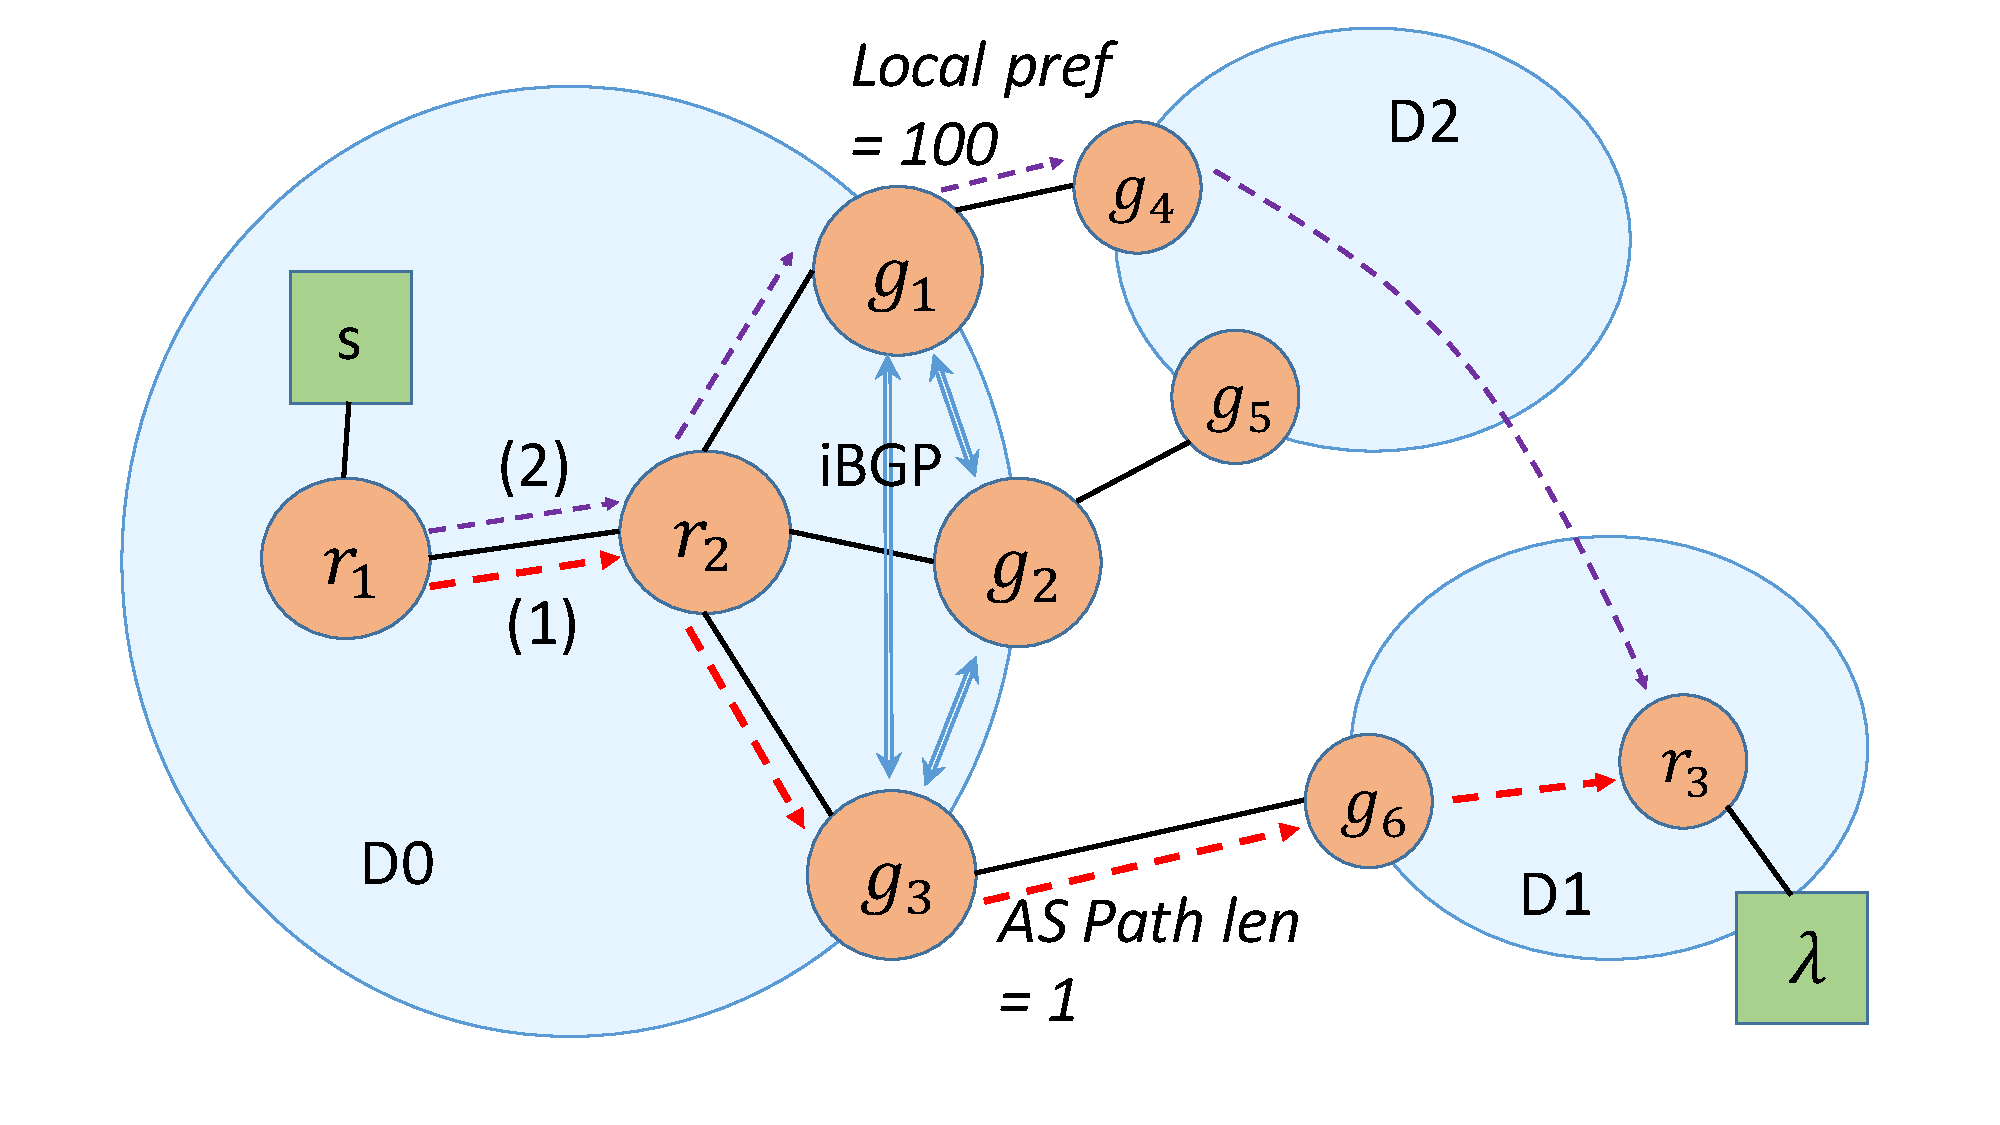
\includegraphics[width=0.66\columnwidth]{figures/bgp-example.pdf}}
	\subfloat[Ex2]{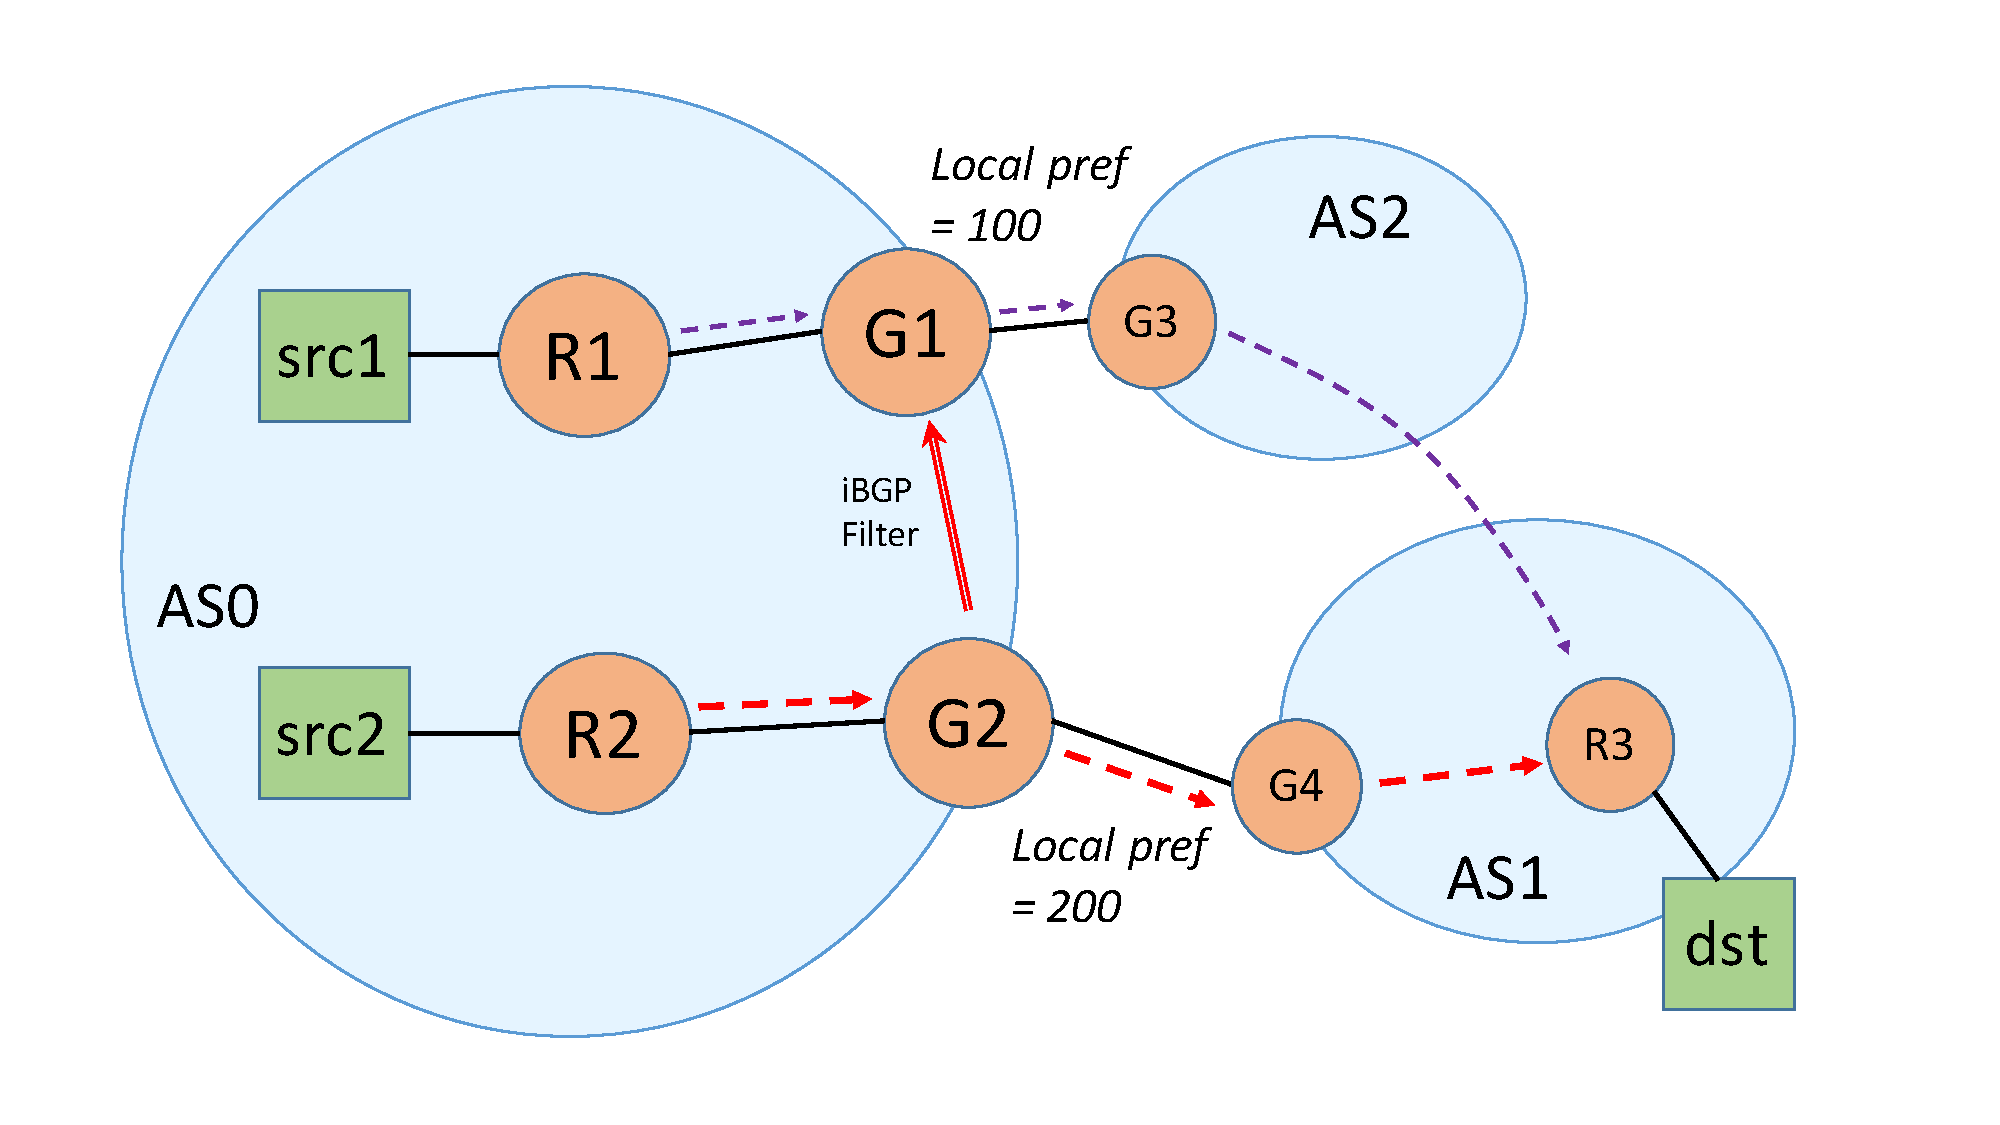
\includegraphics[width=0.6\columnwidth]{figures/bgp-example2.pdf}}
	\subfloat[Ex3]{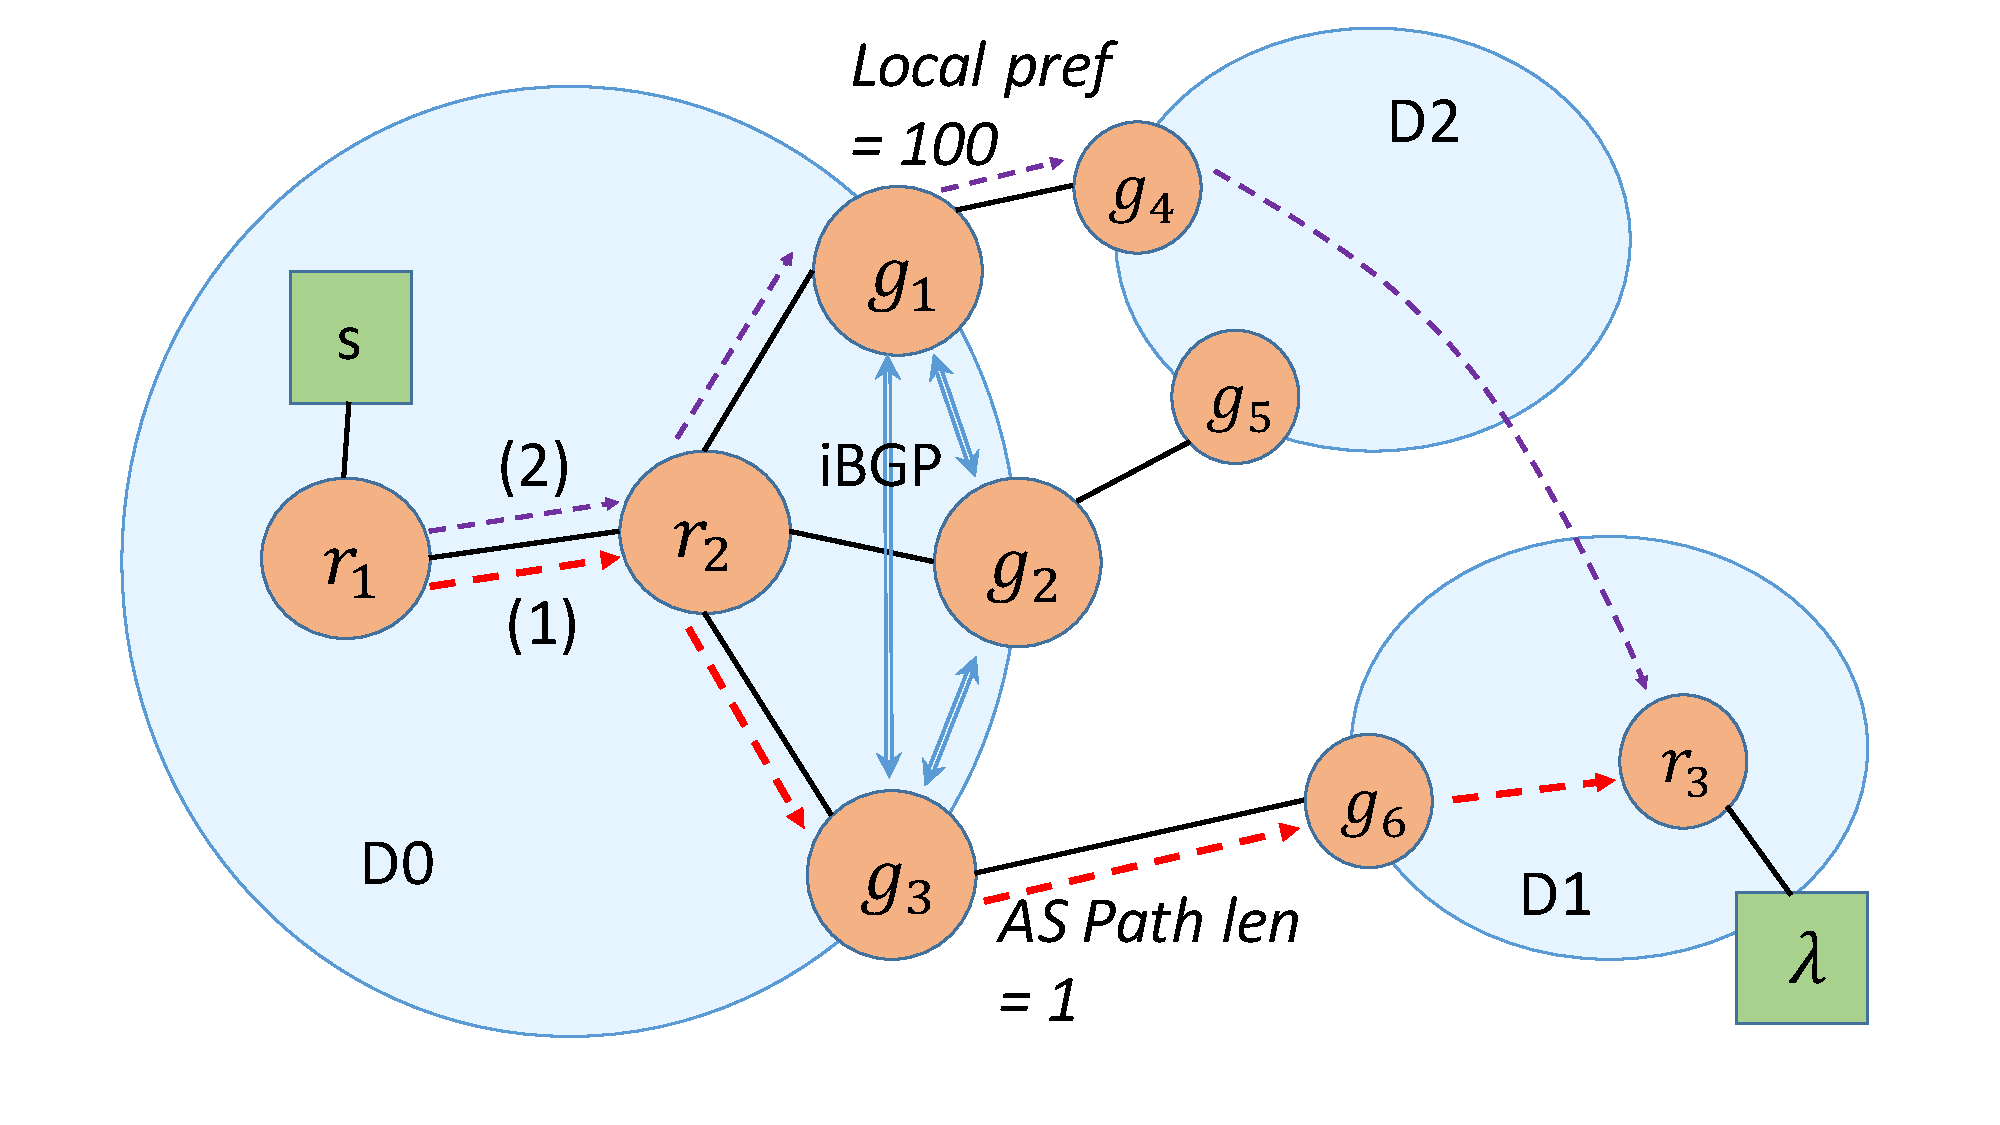
\includegraphics[width=0.66\columnwidth]{figures/bgp-example.pdf}}
	\compactcaption{\label{fig:bgpexample}
	How to configure inter-domain routing}
\end{figure*}

\subsection{BGP configuration}
In \Cref{fig:bgpeg}, we show how \name configures BGP in domain AS0 
to ensure that traffic from $src$ to $dst$ is routed across domains 
such that it follows the path $p$ provided as input. Suppose path (1) is
provided as input. G3 receives a route for $dst$ with AS path length 1
(AS2), while G1 and G2 will receive a route for $dst$ with 
AS path length 2 (AS1, AS2). Since, we need to send traffic along
G3, we do not need to configure any additional BGP variable for $dst$;
\Cref{alg:bgppathrules} will choose the best route for $dst$ 
via G3 (which is the gateway of the input path) as all routes have
the same local preference (0) and AS path length is used to  and $R1$ will
send the packet to $dst$ to G3 along the shortest path (which 
follows the subpath of $p$ from $R1$ to $G3$ by OSPF synthesis). 

Consider the example of input path (2) for $src$ to $dst$ 
in \Cref{fig:bgpeg}. Since, $G1$'s route has a longer AS 
path length greater than $G3$'s route and equal to $G2$'s route,
we need to set the local preference of route received by $G1$ 
(from $G4$) to 100 (any positive value). Thus, \Cref{alg:bgppathrules} 
will select $G1$ as the exit gateway for $dst$. The subpath
$R1$ to $G1$ will be given appropriate weights by the OSPF
synthesis phase so that the synthesizing configurations 
forward traffic along the input path. 

Case 3: Multiple gateways, done using iBGP filters. 

\subsection{Configuration Cost}
\todo{Explain path, as\_path transformation more formally}
\subsubsection{Static Routes} \label{sec:static}
As shown in \Cref{} (Refer to example of 
static routes in motivating example), we require static routes 
to enforce AS paths with loops. Static routes have the lowest 
administrative distance (1) by default~\cite{ad}, and will override BGP
and OSPF routes at a router, this feature can be used to 
exit and enter a domain multiple times. While static routes
do not reduce the resilience of the network (all routes are still
enabled, unlike route-filters), a network under flux will have
unpredictable routing behaviour, unlike with only OSPF and BGP
configured at the routers. 
Also, static routes have to be installed per-destination, thus increasing
the size of configurations drastically as number of policy paths increase.

Given a path $p$ for subnet $\lambda$ and 
the corresponding AS path $p_{as}
= as_1 \rightarrow as_2 \rightarrow \ldots \rightarrow as_m$ (where
$as_m = \Theta(\lambda)$), static
routes are required if $p_{as}$ has a AS-loop. 
To minimize
the number of static routes, we find 
the smallest $i \in [1,m]$ 
such that $\overline{p_{as}} = as_i \rightarrow as_{i+1}
\rightarrow \ldots \rightarrow as_m$ has no loops. 
Therefore, $\overline{p_{as}}$ is the longest AS-loop-free
subpath of $p_{as}$, and be can be enforced using BGP and OSPF. For the 
network path corresponding to AS path $as_1 \rightarrow as_2 
\rightarrow \ldots \rightarrow as_{i-1}$, we require static
routing rules for each next-hop. The static routing score
is the total number of static route hops required to enforce
the input paths.
\todo{Write about the BGP paths are extracted for the next phase}

\subsubsection{BGP Local Preference Entries}
\name uses BGP local preference to route traffic
for a particular subnet to the next AS via a specific 
gateway as per the input paths obtained. 
As shown in \Cref{} (Refer
to ex), if there are multiple exit gateways from an AS 
for a subnet $\lambda$, we require local preference entries at the 
gateways and iBGP filters among these gateways for $\lambda$.

For a domain $d$ and subnet $\lambda$, consider the set 
of paths to $\lambda$ exiting $d$ using BGP (and not statically
routed as described in \Cref{sec:static}). Let $E$ denote the
set of exit gateway routers for the paths of $\lambda$. 
If $|E| = 1$, if gateway $g \in E$ receives a route with 
strictly shortest AS path length (\Cref{alg:bgppathrules}) 
which enforces the paths
for $\lambda$, we do not need to configure local preference
entries on any BGP router in the domain for $\lambda$. If
the exit route chosen by the gateways for $\lambda$ does not 
enforce the paths, \name configures a local preference entry
for $\lambda$ at exit gateway, and thus, the exit route chosen
by BGP enforces the input paths for $\lambda$ in the domain.

If $|E| ~> 1$, multiple BGP routes must be redistributed to 
the OSPF domain. \\
E local prefs + E(E - 1) iBGP filters!

\todo{Changes to OSPF synthesis to ensure closest gateway}
\subsection{Multiple Gateways}
When BGP routes to a destination $\lambda$ 
from multiple gateways are redistributed in
the OSPF domain, \name uses a modified OSPF synthesis
algorithm from \secref{sec:ospfsynthesis}. This is 
required because an OSPF router will choose
the closest BGP gateway in terms of OSPF distance 
for $\lambda$. For instance, a router $r$ will choose
from gateways $g_1$ and $g_2$ according to the $r-g_1$
and $r-g_2$ distance. Therefore, given the input path in
the domain $p=r \rightarrow^+ g1$, \name adds additional
constraints ensuring the distance to $g_2$ from routers
on the path is strictly
greater than the distance to $g_1$ 
on top of the constraints ensuring
$p$ is the shortest path from $r$ to $g_1$. 
Let us define $G_\lambda$ to be the set of gateways
for destination $\lambda$ in the domain. For 
a router $r$, $g \in G_\lambda$ is the gateway if
$r \rightarrow^+_{\xi_{\lambda}} g$ holds, i.e., $g$ 
is reachable from $r$ in the DAG $\xi_{\lambda}$.  
\name adds the following constraints to the 
OSPF synthesis phase to ensure a router
chooses the correct gateway to ensure the input 
paths are induced: 
\begin{multline} \label{eq:gateway}
\forall g \in G_{\lambda}.~\forall r \in \xi_\lambda 
\wedge r \rightarrow^+_{\xi_{\lambda}} g. \\
~\forall g' \in G_{\lambda} \wedge g' \not= g. 
~\forall n' \in N(r) \setminus N_{\xi_\lambda}(r). \\
E(r, n') + D(n', g') > \sum_{\mathclap{\substack{(r_i,r_j) \in r \rightarrow^+_{\xi_{\lambda}} g }}} 
E(r_i, r_j) 
\end{multline}
Like unmodified OSPF synthesis, the system of
constraints generated could be inconsistent and require
route-filters to eliminate constraints. In this scenario,
OSPF needs to filter shorter routes to gateways, and
thus the synthesized configuration would forward traffic to
the gateway specified by the input. We use the same 
approach of picking route-filters from the unsatisfiable core
(\secref{sec:routefilter}), route-filter $((r, n'), \lambda)$
maps to following constraint in the IIS for some $g,g'$: 
\begin{equation}
E(r, n') + D(n', g') > \sum_{\mathclap{\substack{(r_i,r_j) \in r \rightarrow^+_{\xi_{\lambda}} g }}} 
E(r_i, r_j) 
\end{equation}
\todo{abrupt}

\begin{figure}
	\centering
	\begin{tikzpicture}[shorten >=0.5pt,node distance=,on grid,auto,
	square/.style={regular polygon,regular polygon sides=4}] 
	\node[state] at (0,0) [fill=yellow] (s)  {$s$}; 
	\node[state] at (2,0.5) (v1)  {$r_1~~~~$}; 
	\node[state] at (2,-0.5) (u1) {$r_2~~~~$}; 
	\node[state, fill=black!30!green] at (4, 0)(t) {$t$};
	\path[->] 
	(s) edge  node {} (v1)
	edge  node {} (u1)
	edge [blue, dashed, bend right=45] node {} (t)
	edge [red, dashed, bend left=45] node {} (t)
	(u1) edge node {} (t)
	(v1) edge node {} (t);
	\path[-] (u1) edge [dashed] node[above] {} +(0,2);
	\path[-] (v1) edge [dashed] node[above] {} +(0,-2);
	\end{tikzpicture}
	\caption{Diamond}
	\label{fig:diamonddomain}
\end{figure}

\subsection{Route-Filter Cost}
If a diamond created by the input paths (\Cref{fig:diamonddomain}),
\name requires a route-filter to find a solution to OSPF
edge weights. However, if $s$ and $t$ of the diamond lie in
different domains, the inconsistent paths would be split 
across domains, and \name can find OSPF weights for
both the domains without route-filters (in the case if this
diamond was the only source of inconsistency). In the limiting
case where each router is a separate domain~\cite{bgpdatacenter}, 
we do not require any OSPF route-filters, and the entire 
network can be configured using BGP. Thus, a clever domain
assignment can also be reduce the number of route-filters, and
increase the resilience of paths. 


The process of finding the exact static and BGP configurations
required to induce the input paths has polynomial time complexity,
and thus can be found efficiently in every iteration of the MCMC
sampling. To minimize the number of route-filters, we can consider 
the number of route-filters for a given domain assignment $\Theta$ 
as one component of the cost function, and thus MCMC will try
to minimize the cost function, and consequently, the number of
filters. However, finding the optimal number of route-filters for a given domain assignment is NP-hard (\secref{sec:rfcomplexity}), thus, \name
cannot find the exact number of filters for each iteration to use for
the cost function. 

Instead, \name estimates the number of route-filters required for a 
particular domain assignment $\Theta$ for the cost function. Before 
we start the MCMC search, we undergo a preprocessing phase 
where for every pair of input paths, we identify the
number of diamonds created by the path (\todo{define diamond 
	formally somewhere}) and store the start and end router of 
each diamond. In a MCMC iteration based on the domain
assignment $\Theta$, for every diamond, we check if the
start and end router are part of the same domain. If yes, 
we assume we require atleast one filter for this particular
diamond and increment the route-filter cost by 1. The 
route-filter cost is not increment if the start and end 
router of the diamond belong in different domains in $\Theta$.

The cost computed by the above procedure overestimates the
number of route-filters required to eliminate the diamonds.  
Two different diamonds sharing an edge could be both 
eliminated by a single filter, whereas our route-filter cost 
would be 2. However, there are path fragments which 
lead to inconsistencies, but are not diamonds, and thus
are not included in the route-filter cost. However, the 
cost can be computed efficiently every iteration, and 
our experiments show reductions in route-filter cost 
lead to reductions in number of filters(~\Cref{some experiment}). 
\todo{Specify weird Route filter case without diamonds?}







